

%\documentclass[pra,twocolumn,epsfig,rotate,superscriptaddress,showpacs]{revtex4}


% \mathcal{u}se only LaTeX2e, calling the article.cls class and 12-point type.

\documentclass[prl,onecolumn]{revtex4-1}
\usepackage{graphicx}
\usepackage{epsfig}
\usepackage{epsf}
\usepackage{amssymb}
\usepackage{amsmath}
\usepackage{amsthm}
\usepackage{multirow}
\usepackage{hyperref}

\usepackage[framed,numbered]{matlab-prettifier}
\let\ph\snippetPlaceholder
\lstset
{
  style = Matlab-editor,
  escapechar      = ",
}

\renewcommand{\familydefault}{\sfdefault}  %% arial font
% \usepackage{times} %% times new roman font

\newcommand{\bra}[1]{\langle #1|}
\newcommand{\ket}[1]{|#1\rangle}
\newcommand{\dir}{$\backslash$}
\newcommand{\be}{\begin{equation}}
\newcommand{\ee}{\end{equation}}
\newcommand{\bea}{\begin{eqnarray}}
\newcommand{\eea}{\end{eqnarray}}
\newcommand{\Fig}[1]{Fig.\,\ref{#1}}
\newcommand{\Eq}[1]{Eq.\,(\ref{#1})}
\newcommand{\la}{\langle}
\newcommand{\ra}{\rangle}
\newcommand{\nl}{\nonumber \\}
%\usepackage[usenames]{color}
%\definecolor{Red}{rgb}{1,0,0}
%\definecolor{Blue}{rgb}{0,0,1}




\setlength{\parindent}{0pt} % no incident
%\renewcommand{\baselinestretch}{1.2} % space between two lines
\setlength{\parskip}{6\lineskip} % space between two paragraphs

%%%%%%%%%%%%%%%%% END OF PREAMBLE %%%%%%%%%%%%%%%%



\begin{document}

% Include your paper's title here
\title{Code updating history of Jump Code Experiment}
\author{Dawei Lu}

\begin{abstract}
Notes about the Matlab code used in the Jump Code Experiments.
\end{abstract}
\today

\maketitle

\section{Background (Apr 07, 2015)}

All the codes are available in SVN 'https:\dir \dir github.com\dir bannislloyd\dir dawei-qip-matlab\dir trunk\dir Jump Code'

The flipping error channel and erasing error channel are 
\be
A_0 = \left(
         \begin{array}{cc}
           1 & 0 \\
           0 & \sqrt{1-r} \\
         \end{array}
       \right),
A_1 = \left(
         \begin{array}{cc}
           0 & 0 \\
           0 & \sqrt{r} \\
         \end{array}
       \right),       
\ee

Since $A_0 = [(1+\sqrt{1-r})/2]I+[(1-\sqrt{1-r})/2]Z$, we know in the Hadamard basis the qubit will be flipped with the probability 
\be
p_F = [(1-\sqrt{1-r})/2]^2,
\ee
and no error probability 
\be
p_0 = [(1+\sqrt{1-r})/2]^2.
\ee
And $A_1\ket{+}=\sqrt{r/2}\ket{1}, A_1\ket{-}=-\sqrt{r/2}\ket{1}$, so $A_1$ will erase all the information in the Hadamard basis with the probability $p_E = r/2$.

To make a unitary transformation, we need one ancilla. Assume the ancilla starts at $\ket{0}$, so we can use the following way to construct unitary. The channel $\Phi$ on these 2 qubits (ancilla A and system B) should give us
\be
\Phi(\rho_{AB}) = \ket{0}\bra{0}\otimes A_0\rho_BA_0^{\dagger} +\ket{1}\bra{1} \otimes A_1\rho_BA_1^{\dagger}.
\ee
$\Phi$ is not unitary but we can use a unitary channel $U$ with the aid of post selection to realize it. It means if we start from $\ket{00}$ and $\ket{01}$ (Note we have assumed the ancilla A is from $\ket{0}$), by applying $U$ we will have
\be
U\ket{00} = \ket{00}, U\ket{01} = \sqrt{1-r}\ket{01}+\sqrt{r}\ket{11}.
\ee
So the unitary can be chosen in this way
\be
U = \left(
      \begin{array}{cccc}
        1 & 0 & 0 & 0 \\
        0 & \sqrt{1-r} & 0 & \sqrt{r} \\
        0 & 0 & -1 & 0 \\
        0 & \sqrt{r} & 0 & -\sqrt{1-r} \\
      \end{array}
    \right).
\ee

In summary, we have three probabilities 
\bea
p_0 &=& [(1+\sqrt{1-r})/2]^2, \nonumber \\ 
p_F &=& [(1-\sqrt{1-r})/2]^2, \nonumber \\
p_E &=& r/2.
\eea

\section{Classical Case Without Correction (Apr 07, 2015)}
First consider the classical case. Without correction, one needs one bit with the two states $\ket{+}$ or $\ket{-}$. Suppose it is $\ket{+}$.

We can use 2 qubits (ancilla and system) starting from $\ket{0+}$. Applying $U$ and post-select the ancilla. If we get $\ket{0}$, we know $A_0$ happens and with probability $p_0$ no error happens, with probability $p_F$ $\ket{+}$ is flipped to $\ket{-}$. If we get $\ket{1}$, we know $A_1$ happens (the probability of this case is $p_E$) and we will get $\ket{1}$ on the system. We have half chance to recover it to the correct state $\ket{+}$. Therefore, the fidelity for this classical case will be 
\be
F^C = p_0+\frac{1}{2}p_E = \frac{1}{2}+\frac{1}{2}\sqrt{1-r}
\ee

The matlab code is (for a given $r$)
\begin{lstlisting}
% projective measurement
M0 = kron(ST0, I); M1 = kron(ST1, I);

rho_projective0 = M0*rho_channel*M0'; % if ST0 is detected on the ancilla
% equal to  rho_echo = Gz_echo(rho_channel,2), simulated by Gradient Echo
rho_sys0 = ptrace(rho_projective0, 1, [2 2]); % trace out ancilla
Fidelity0 = trace(System*rho_sys0);

rho_projective1 = M1*rho_channel*M1';  % if ST1 is detected on the ancilla
% equal to  rho_echo = Gz_echo(rho_channel,2), simulated by Gradient Echo
rho_sys1 = ptrace(rho_projective1, 1, [2 2]); % trace out ancilla
Fidelity1 = trace(System*rho_sys1); 
\end{lstlisting}

The total fidelity is Fidelity0+Fidelity1 and equals to $F^C$.

\section{Classical Case With Correction (Apr 07, 2015)}
Without correction, one needs two bits with the two states $\ket{++}$ or $\ket{--}$ to encode one bit information. Suppose it is $\ket{++}$.

We have to use 4 qubits (ancilla, system, system, ancilla) to simulate this case. Applying $U$ and post-select the 2 ancillas.

\textbf{Case 1:} If we get $\ket{00}$, we know $A_0A_0$ happens. We have $p_0^2$ probability for no error and $p_F^2$ for flip error on both qubits. The latter one cannot be corrected. Besides, we have $2p_0p_F$ probability that only one flip error happens. So we can project the system to $\{\ket{++}, \ket{+-}, \ket{-+}, \ket{--}\}$ basis. If we get $\ket{++}$ or $\ket{--}$, do nothing. If we get $\ket{+-}$ or $\ket{-+}$, discard the 2nd qubit and use the 1st qubit state as the real one. It means we have $p_0p_F$ probability to succeed, and $p_Fp_0$ probability to fail. In total, for Case 1, the succeeding probability is $p_0^2+p_0p_F$.

\textbf{Case 2:} If we get $\ket{01}$, we know $A_0A_1$ happens. Discard the 2nd qubit and use the 1st qubit state. The succeeding probability is thus $p_0p_E$.

\textbf{Case 3:} If we get $\ket{10}$, we know $A_1A_0$ happens. Discard the 1st qubit and use the 2nd qubit state. The succeeding probability is thus $p_Ep_0$.

\textbf{Case 4:} If we get $\ket{11}$, we know $A_1A_1$ happens. The final result would be $\ket{11}$ on the system and we have half chance to get the correct state $\ket{++}$. The probability is thus $\frac{1}{2}p_E^2$.

The total fidelity with error correction in the classical case will be 
\be
F^C_{code} = p_0^2+p_0p_F+p_0p_E+p_Ep_0+ \frac{1}{2}p_E^2.
\ee

Comparing the classical case with and without error correction, we will have the following figure. And we know for any $r$, the error correction performs better than the original case.

\begin{figure}[!h]
\begin{center}
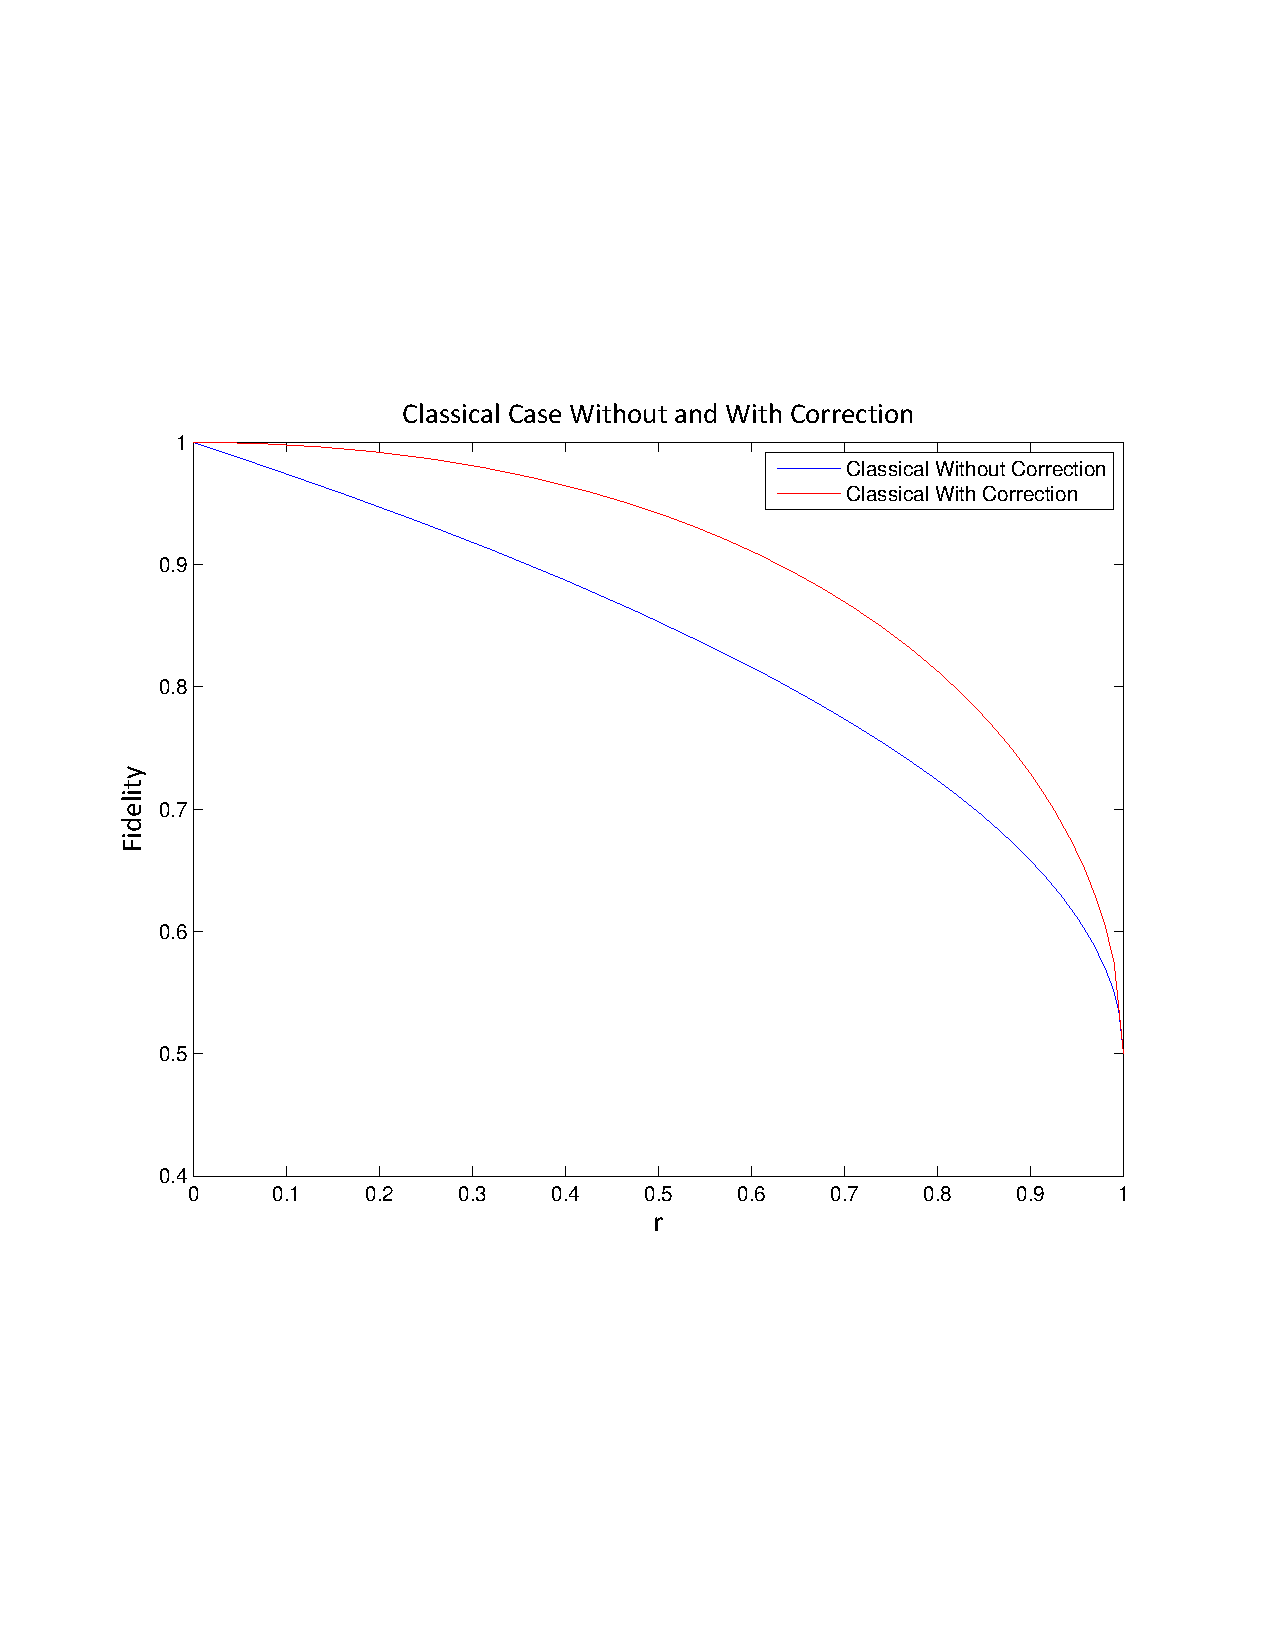
\includegraphics[width=\columnwidth]{Classical.pdf}
\end{center}
\setlength{\abovecaptionskip}{-0.35cm}
\caption{\footnotesize{Classical case with and without error correction.}}\label{classical}
\end{figure}

\begin{thebibliography}{99}
%\bibitem{Moussa2012} O. Moussa, M. da Silva, C. Ryan, and R. Laflamme, Phys. Rev. Lett. \textbf{109}, 070504 (2012).

\end{thebibliography}


\end{document}
